\documentclass[compress]{beamer}        % [compress] (written before {beamer} <=> navigation bar one line, all subsections in 1 line instead of 2

% Setup appearance:
\usetheme{CambridgeUS}
%	AnnArbor | Antibes | Bergen |
%	Berkeley | Berlin | Boadilla |
%	boxes | CambridgeUS | Copenhagen |
%	Darmstadt | default | Dresden |
%	Frankfurt | Goettingen |Hannover |
%	Ilmenau | JuanLesPins | Luebeck |
%	Madrid | Malmoe | Marburg |
%	Montpellier | PaloAlto | Pittsburgh |
%	Rochester | Singapore | Szeged |
%	Warsaw
%

\useoutertheme[footline=authorinstitute,subsection=false]{miniframes}
\usecolortheme{whale}

%	albatross | beaver | beetle |
%	crane | default | dolphin |
%	dove | fly | lily | orchid |
%	rose |seagull | seahorse |
%	sidebartab | structure |
%	whale | wolverine


\setbeamertemplate{footline}
{
  \hbox{%
  \begin{beamercolorbox}[wd=.25\paperwidth,ht=2.25ex,dp=1ex,center]{title in head/foot}%
    \usebeamerfont{date in head/foot}\insertshortauthor
  \end{beamercolorbox}%
  \begin{beamercolorbox}[wd=.5\paperwidth,ht=2.25ex,dp=1ex,center]{date in head/foot}%
    \usebeamerfont{title in head/foot}\insertshortinstitute
  \end{beamercolorbox}%
  \begin{beamercolorbox}[wd=.25\paperwidth,ht=2.25ex,dp=1ex,center]{title in head/foot}%
    \usebeamerfont{date in head/foot}
    \insertframenumber{} / \inserttotalframenumber
  \end{beamercolorbox}}%
  \vskip0pt%
}

%\setbeamercolor{titlelike}{parent=structure}
%\setbeamercolor{structure}{fg=beamer@blendedblue}
%% \useinnertheme{rounded}
%\setbeamerfont{block title}{size={}}
%\usefonttheme[onlylarge]{structurebold}   % title and words in the table of contents bold
%\setbeamerfont*{frametitle}{size=\normalsize,series=\bfseries}
\setbeamertemplate{navigation symbols}{}
\setbeamercolor{frametitle}{parent=boxes, bg=white}


% Standard packages

\usepackage[english]{babel}
\usepackage[latin1]{inputenc}
\usepackage{times}
\usepackage[T1]{fontenc}
\usepackage{amsbsy}         % for \boldsymbol command (bold in math mode)
\usepackage{amsfonts, amssymb}
\usepackage{epsfig}
\usepackage{color}
\definecolor{camblue}{RGB}{26,26,89}
\definecolor{Rblue}{RGB}{0,255,255}
\definecolor{Rdarkblue}{RGB}{0,0,255}
\definecolor{Rgreen}{RGB}{0,205,0}
\newcommand{\tcb}{\textcolor{beamer@blendedblue}}
\newcommand{\tcbb}{\textcolor{camblue}}
\newcommand{\tcr}{\textcolor{red}}
\newcommand{\tcg}{\textcolor{gray}}
\newcommand{\tcRg}{\textcolor{Rgreen}}
\newcommand{\tcRdb}{\textcolor{Rdarkblue}}
\newcommand{\tcRb}{\textcolor{Rblue}}
\newcommand{\sq}{\begin{eqnarray}}
\newcommand{\fq}{\end{eqnarray}}
\newcommand{\bp}{$\bullet$\:}


%%%%%%%%%%%%%%%%%%%%%%%%%%%%%%%%%%%%%%%%%%%%%%%%%%%%%%%%%%%%%%%%%%%%%%%%%%%%%%%%%%%%%%%%%%%%%
% THIS IS WHERE THE DOCUMENT BEGINS


%\setbeamercovered{transparent}   % overlays with light grey 1st slide
\title
{
{\huge Title\\[0.3cm] }
}
\author[Kevin O'Brien]{{\bf Author}}
\institute[University of Limerick, Maths \& Stats Dept]{}
\date{}

\begin{document}
\section{Bland-Altman Methods}



%------------------------------------------------------------------------%












%%%%%%%%%%%%%%%%%%%%%%%%%%%%%%%%%%%%%%%%%%%%%%%%%%%%%%%%%%%%%%%%%%%%%%%%%%%%%%%%%%%%%%

\subsection{Bland-Altman Difference Plot}
%%%%%%%%%%%%%%%%%%%%%%%%%%%%%%%%%%%%%%%%%%%%%%%%%%%%%%%%%%%%%%%%%%%%%%%%%%%%%%%%%%%%%%
\begin{frame}
\frametitle{Some Key Concepts}
\begin{itemize}
\item In clinical measurement comparison of a new measurement technique with an established one is often needed to see whether they \textbf{\textit{agree}} sufficiently for the new to replace the old. [2]
\item 
A method comparison study is
a study where two methods of quantitative measurement are compared by measuring the
same set of items with both methods.

\end{itemize}
\end{frame}
%%%%%%%%%%%%%%%%%%%%%%%%%%%%%%%%%%%%%%%%%%%%%%%%%%%%%%%%%%%%%%%%%%%%%%%%%%%%%%%%%%%%%%
\begin{frame}
\frametitle{Bland-Altman Plots}
\large
\begin{itemize}
%\item 
%The issue of whether two measurement methods comparable to the
%extent that they can be used interchangeably with sufficient
%accuracy is encountered frequently in scientific research.
\item Historically comparison of two methods of measurement was carried
out by use of paired sample t-test, correlation coefficients or
simple linear regression.
\item  Statisticians Martin Bland and Douglas
Altman recognized the inadequacies of these analyses and
articulated quite thoroughly the basis on which of which they are
unsuitable for comparing two methods of measurement [1].

\end{itemize}
\end{frame}
%%%%%%%%%%%%%%%%%%%%%%%%%%%%%%%%%%%%%%%%%%%%%%%%%%%%%%%%%%%%%%%%%%%%%%%%%%%%%%%%%%%%%%
\begin{frame}
\frametitle{Using Bland-Altman Plots}
Bland-Altman plots are a powerful graphical methodology for making
a visual assessment of the data. Bland and Altman [1] express the
motivation for this plot thusly:
\begin{quote}
``From this type of plot it is much easier to assess the magnitude
of disagreement (both error and bias), spot outliers, and see
whether there is any trend, for example an increase in
(difference) for high values. This way of plotting the data is a
very powerful way of displaying the results of a method comparison
study."
\end{quote}
\end{frame}

%%%%%%%%%%%%%%%%%%%%%%%%%%%%%%%%%%%%%%%%%%%%%%%%%%%%%%%%%%%%%%%%%%%%%%%%%%%%%%%%%%%%%%
\begin{frame}
\frametitle{Bland-Altman Plots}
\large
\begin{itemize}
\item 
Furthermore they proposed their simple methodology specifically
constructed for method comparison studies. 
\item They acknowledge the
opportunity to apply other valid, but complex, methodologies, but
argue that a simple approach is preferable, especially when the
results must be `\textit{explained to non-statisticians}'.
\end{itemize}
\end{frame}

%----------------------------------------------------------------- %
\begin{frame}{\bf \tcb{The Bland-Altman Plot}}
\begin{itemize}\itemsep0.4cm

\item The Bland-Altman plot [1,2,3] is a very simple graphical method to compare two measurements techniques. \item In this approach the case-wise differences between the two methods are plotted against the corresponding case-wise averages of the two methods.
\item As the
objective of the Bland-Altman plot is to advise on the agreement
of two methods, it is the case-wise differences that are
particularly important. 
\item A horizontal lines is drawn at the mean difference(the inter-method bias) , and at the \textbf{\textit{limits of agreement}}, which are defined as the inter-method bias plus and minus 2 times the standard deviation of the differences.
\end{itemize}
\end{frame}

%\begin{frame}
%\begin{itemize}
%\item The Bland-Altman plot is simply a scatterplot of the case-wise
%averages and differences of two methods of measurement. 
%
%\item Later it will be shown that case-wise differences
%are the sole component of the next part of the methodology, the
%limits of agreement.
%\end{itemize}

%\end{frame}
%%%%%%%%%%%%%%%%%%%%%%%%%%%%%%%%%%%%%%%%%%%%%%%%%%%%%%%%%%%%%%%%%%%%%%%%%%%%%%%%%%%%%%
\begin{frame}

\begin{itemize}
\item For creating plots, the case wise-averages fulfil several
functions, such as expressing the range over which the values were
taken, and assessing whether the assumptions of constant variance
holds.
\item Case-wise averages also allow the case-wise differences to
be presented on a two-dimensional plot, with better data
visualization qualities than a one dimensional plot.
\item\textit{ Bland \& Altman [2]
cautions that it would be the difference against either
measurement value instead of their average , as the difference
relates to both value.}
\end{itemize}
\end{frame}

%%%%%%%%%%%%%%%%%%%%%%%%%%%%%%%%%%%%%%%%%%%%%%%%%%%%%%%%%%%%%%%%%%%%%%%%%%%%%%%%%%%%%%
\begin{frame}
\large
\begin{itemize}
\item The magnitude of the \textbf{\textit{inter-method bias}} between the two methods is
simply the average of the differences $\bar{d}$.
\item The variances
around this bias is estimated by the standard deviation of the
differences $S(d)$. 
\item This inter-method bias is represented with a
line on the Bland-Altman plot. 
\item These estimates are only meaningful
if there is uniform inter-bias and variability throughout the
range of measurements, which can be checked by visual inspection
of the plot.
\end{itemize}
 
\end{frame}

\subsection*{R Code}
%-------------------------------------------------------------------%
\begin{frame}[fragile]
\frametitle{Bland-Altman Plot}
\begin{verbatim}
>X = rnorm(14,6,1);Y = rnorm(14,5.3,1.1)
>
>A=(X+Y)/2		#case-wise averages
>D=X-Y			#case-wise differences
>		
>Dbar=mean(D)	#inter-method bias
>SdD=sd(D)		#standard deviation of the differences
>
>plot(A,D,pch=16,col="red", ylim=c(-3,3))
>
>abline(h=Dbar,lty=2)
>abline(h=(Dbar-2*SdD),lty=2)
>abline(h=(Dbar+2*SdD),lty=2)
\end{verbatim}
\end{frame}


\begin{frame}
\frametitle{Simple Bland-Altman Plot}
Inter-method Bias : 0.45 | Limits of Agreement: [-1.32, 2.23]
\vspace{0.5cm}
\begin{center}
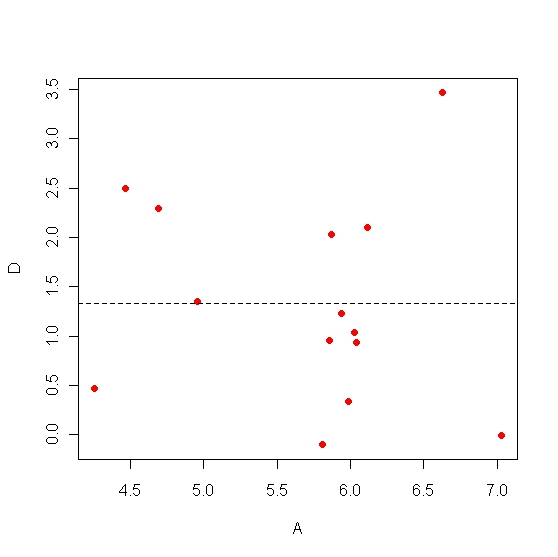
\includegraphics[scale = 0.30]{SimpleBAplot}
\end{center}
\end{frame}






%%%%%%%%%%%%%%%%%%%%%%%%%%%%%%%%%%%%%%%%%%%%%%%%%%%%%%%%%%%%%%%%%%%%%%%%%%%%%%%%%%%%%%%
%\begin{frame}
%\frametitle{The Bland-Altman Difference Plot}
%\begin{itemize}
%\item In light of shortcomings associated with scatterplots,
%\alert{BA83} recommend a further analysis of the data. 
%\item Firstly
%case-wise differences of measurements of two methods $d_{i} =
%y_{1i}-y_{2i} \mbox{ for }i=1,2,..n$ on the same subject should be
%calculated, and then the average of those measurements ($a_{i} =
%(y_{1i} + y_{2i})/2 \mbox{ for }i=1,2,..n$). 
%\item These differences and
%averages are then plotted. 
%\end{itemize}
%
%\end{frame}








%------------------------------------------------------------------------------%

% Breaking assumptions - using CS and Symmetric VCs
% LRT implemented using "anova" function
% JSR Blood data

%------------------------------------------------------------------------------%


%%%%%%%%%%%%%%%%%%%%%%%%%%%%%%%%%%%%%%%%%%%%%%%%%%%%%%%%%%%%%%%%%%%%%%%%%%%%%%%%%%%%%%


%%%%%%%%%%%%%%%%%%%%%%%%%%%%%%%%%%%%%%%%%%%%%%%%%%%%%%%%%%%%%%%%%%%%%%%%%%%%%%%%%%%%%%
\section{Grubbs - Data Example}

%%%%%%%%%%%%%%%%%%%%%%%%%%%%%%%%%%%%%%%%%%%%%%%%%%%%%%%%%%%%%%%%%%%%%%%%%%%%%%%%%%%%%%
\begin{frame}
\begin{table}[h!]

\begin{center}
\begin{tabular}{|c||c|c||c|c|}
  \hline
 Round & Fotobalk  & Counter  & Differences  & Averages  \\
  &  [F] & [C] & [F-C] &  [(F+C)/2] \\
  \hline \hline
  
1 & 793.8 & 794.6 & -0.8 & 794.2 \\
  2 & 793.1 & 793.9 & -0.8 & 793.5 \\
  3 & 792.4 & 793.2 & -0.8 & 792.8 \\
  4 & 794.0 & 794.0 & 0.0 & 794.0 \\
  5 & 791.4 & 792.2 & -0.8 & 791.8 \\
  6 & 792.4 & 793.1 & -0.7 & 792.8 \\
  7 & 791.7 & 792.4 & -0.7 & 792.0 \\
  8 & 792.3 & 792.8 & -0.5 & 792.5 \\
  9 & 789.6 & 790.2 & -0.6 & 789.9 \\
  10 & 794.4 & 795.0 & -0.6 & 794.7 \\
  11 & 790.9 & 791.6 & -0.7 & 791.2 \\
  12 & 793.5 & 793.8 & -0.3 & 793.6 \\
   \hline
\end{tabular}
\caption{Fotobalk and Counter methods: differences and averages.}
\end{center}
\end{table}
\end{frame}
%%%%%%%%%%%%%%%%%%%%%%%%%%%%%%%%%%%%%%%%%%%%%%%%%%%%%%%%%%%%%%%%%%%%%%%%%%%%%%%%%%%%%%
\begin{frame}
\begin{table}[h!]

\begin{center}
\begin{tabular}{|c||c|c||c|c|}
  \hline
 Round & Fotobalk  & Terma  & Differences  & Averages  \\
  &  [F] & [T] & [F-T] &  [(F+T)/2] \\
  \hline
1 & 793.80 & 793.20 & 0.60 & 793.50 \\
  2 & 793.10 & 793.30 & -0.20 & 793.20 \\
  3 & 792.40 & 792.60 & -0.20 & 792.50 \\
  4 & 794.00 & 793.80 & 0.20 & 793.90 \\
  5 & 791.40 & 791.60 & -0.20 & 791.50 \\
  6 & 792.40 & 791.60 & 0.80 & 792.00 \\
  7 & 791.70 & 791.60 & 0.10 & 791.65 \\
  8 & 792.30 & 792.40 & -0.10 & 792.35 \\
  9 & 789.60 & 788.50 & 1.10 & 789.05 \\
  10 & 794.40 & 794.70 & -0.30 & 794.55 \\
  11 & 790.90 & 791.30 & -0.40 & 791.10 \\
  12 & 793.50 & 793.50 & 0.00 & 793.50 \\

   \hline
\end{tabular}
\caption{Fotobalk and Terma methods: differences and averages.}
\end{center}
\end{table}
\end{frame}

%%%%%%%%%%%%%%%%%%%%%%%%%%%%%%%%%%%%%%%%%%%%%%%%%%%%%%%%%%%%%%%%%%%%%%%%%%%%%%%%%%%%%%
\begin{frame}
\frametitle{Grubbs Data - Identity Plot}
\large
\begin{itemize}
\item Notwithstanding previous remarks about regression, the first step
recommended, which the authors argue should be mandatory, is
construction of a simple scatter plot of the data. 
\item The \textbf{\textit{line of
equality}} must also be shown, as it is necessary to give the
correct interpretation of how both methods compare. 
\item A scatter plot
of the Grubbs data (forthcoming example) is shown in Figure 1.1. 
\item Visual inspection confirms the previous conclusion that there is an
inter-method bias present, i.e. Fotobalk device has a tendency to
record a lower velocity.
\end{itemize}
\end{frame}
%%%%%%%%%%%%%%%%%%%%%%%%%%%%%%%%%%%%%%%%%%%%%%%%%%%%%%%%%%%%%%%%%%%%%%%%%%%%%%%%%%%%%%
\begin{frame}
\frametitle{Grubbs Data - Identity Plot}
\begin{figure}[h!]
\begin{center}
  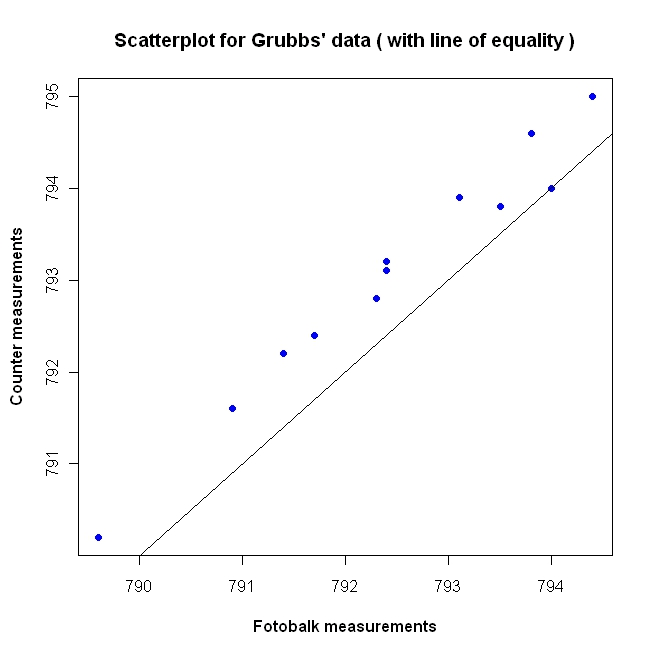
\includegraphics[width=80mm]{GrubbsScatter.jpeg}
  \caption{Scatter plot For Fotobalk and Counter Methods.}\label{GrubbsScatter}
\end{center}
\end{figure}
\end{frame}


\begin{frame}
\large
\textbf{Grubbs Example}
\begin{itemize}
\item 
In the case of Grubbs data the inter-method bias is
$-0.61$ metres per second, and is indicated by the dashed line on
Figure 1.2. 
\item By inspection of the plot, it is also possible to
compare the precision of each method. 
\item Noticeably the differences
tend to increase as the averages increase.
\end{itemize}
\end{frame}

\subsection{Interpreting Bland-Altman Plots}


%%%%%%%%%%%%%%%%%%%%%%%%%%%%%%%%%%%%%%%%%%%%%%%%%%%%%%%%%%%%%%%%%%%%%%%%%%%%%%%%%%%%%%
\begin{frame}
\textbf{Next Slide}
\begin{itemize}
\item The Bland-Altman plot for comparing the `Fotobalk' and `Counter'
methods, which shall henceforth be referred to as the `F vs C'
comparison,  is depicted in Figure 1.2, using data from Table 1.3.
\item The presence and magnitude of the inter-method bias is indicated
by the dashed line.
\end{itemize}
\end{frame}
%%%%%%%%%%%%%%%%%%%%%%%%%%%%%%%%%%%%%%%%%%%%%%%%%%%%%%%%%%%%%%%%%%%%%%%%%%%%%%%%%%%%%%
\begin{frame}
\begin{figure}[h!]
\begin{center}
  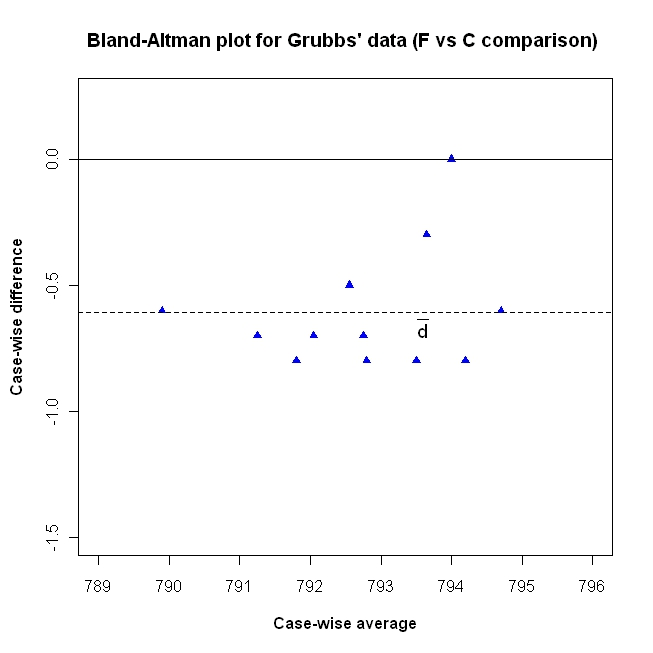
\includegraphics[width=70mm]{GrubbsBAplot-noLOA.jpeg}
  \caption{Bland-Altman plot For Fotobalk and Counter methods.}\label{GrubbsBA-noLOA}
\end{center}
\end{figure}
\end{frame}
%%%%%%%%%%%%%%%%%%%%%%%%%%%%%%%%%%%%%%%%%%%%%%%%%%%%%%%%%%%%%%%%%%%%%%%%%%%%%%%%%%%%%%
\begin{frame}
\textbf{Next Slide}

In the next slide Bland-Altman plots for the `F vs C' and `F vs T'
comparisons are shown, where `F vs T' refers to the comparison of
the `Fotobalk' and `Terma' methods. Usage of the Bland-Altman plot
can be demonstrate in the contrast between these comparisons.
\end{frame}
%%%%%%%%%%%%%%%%%%%%%%%%%%%%%%%%%%%%%%%%%%%%%%%%%%%%%%%%%%%%%%%%%%%%%%%%%%%%%%%%%%%%%%
\begin{frame}

\begin{figure}[h!]
\begin{center}
  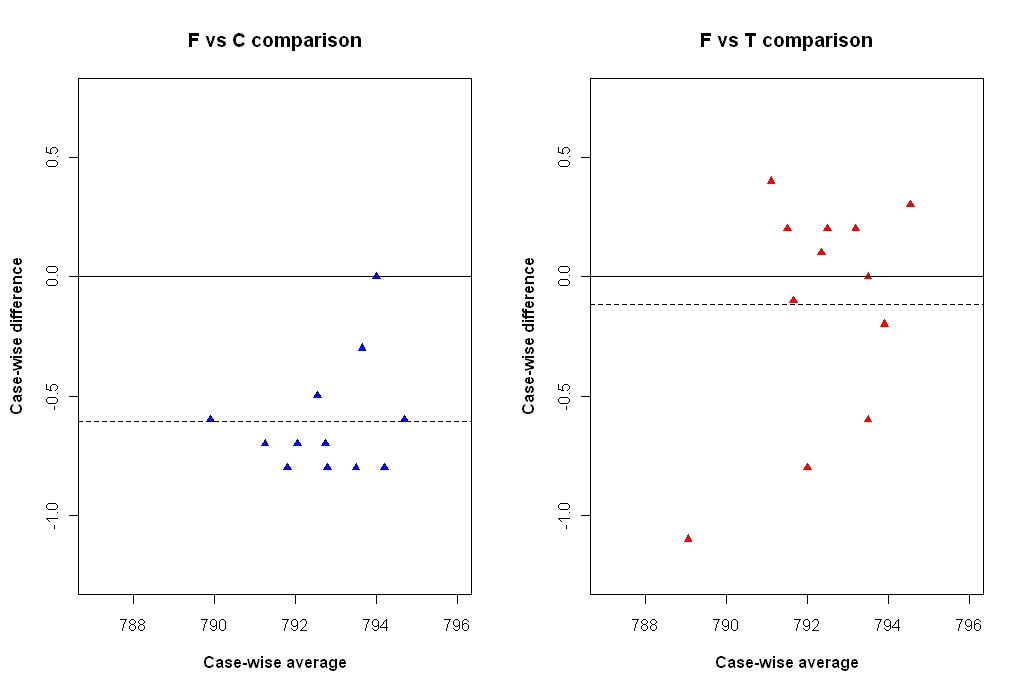
\includegraphics[height=80mm]{GrubbsDataTwoBAplots.jpeg}
  \caption{Bland-Altman plots for Grubbs' F vs C and F vs T comparisons.}\label{GrubbsDataTwoBAplots}
\end{center}
\end{figure}
\end{frame}
%%%%%%%%%%%%%%%%%%%%%%%%%%%%%%%%%%%%%%%%%%%%%%%%%%%%%%%%%%%%%%%%%%%%%%%%%%%%%%%%%%%%%%
\begin{frame}
\begin{itemize}
\item By inspection, there exists a larger inter-method bias in the `F
vs C' comparison than in the `F vs T' comparison. 
\item Conversely there
appears to be less precision in`F vs T' comparison, as indicated
by the greater dispersion of co-variates.


\end{itemize}

\end{frame}

%%%%%%%%%%%%%%%%%%%%%%%%%%%%%%%%%%%%%%%%%%%%%%%%%%%%%%%%%%%%%%%%%%%%%%%%%%%%%%%%%%%%%%
\begin{frame}
\frametitle{Interpreting Bland-Altman Plots}
\begin{itemize}

\item In the following slides are some prototype Bland-Altman plots
derived from simulated data, each for the purpose of demonstrating
how the plot would inform an analyst of features that would
adversely affect use of the recommended methodology.
\end{itemize}

\end{frame}
%%%%%%%%%%%%%%%%%%%%%%%%%%%%%%%%%%%%%%%%%%%%%%%%%%%%%%%%%%%%%%%%%%%%%%%%%%%%%%%%%%%%%%
%\begin{frame}
%Figure 1.4 demonstrates how the Bland-Altman plot would indicate
%increasing variance of differences over the measurement range.
%Fitted regression lines, for both the upper and lower half of the
%plot, has been added to indicate the trend. Figure 1.5 is an
%example of cases where the inter-method bias changes over the
%measurement range. This is known as proportional bias. In both
%Figures 1.4 and 1.5, the assumptions necessary for further
%analysis using the limits of agreement are violated.
%\end{frame}

%%%%%%%%%%%%%%%%%%%%%%%%%%%%%%%%%%%%%%%%%%%%%%%%%%%%%%%%%%%%%%%%%%%%%%%%%%%%%%%%%%%%%%
\begin{frame}
\begin{figure}[h!]
\begin{center}
  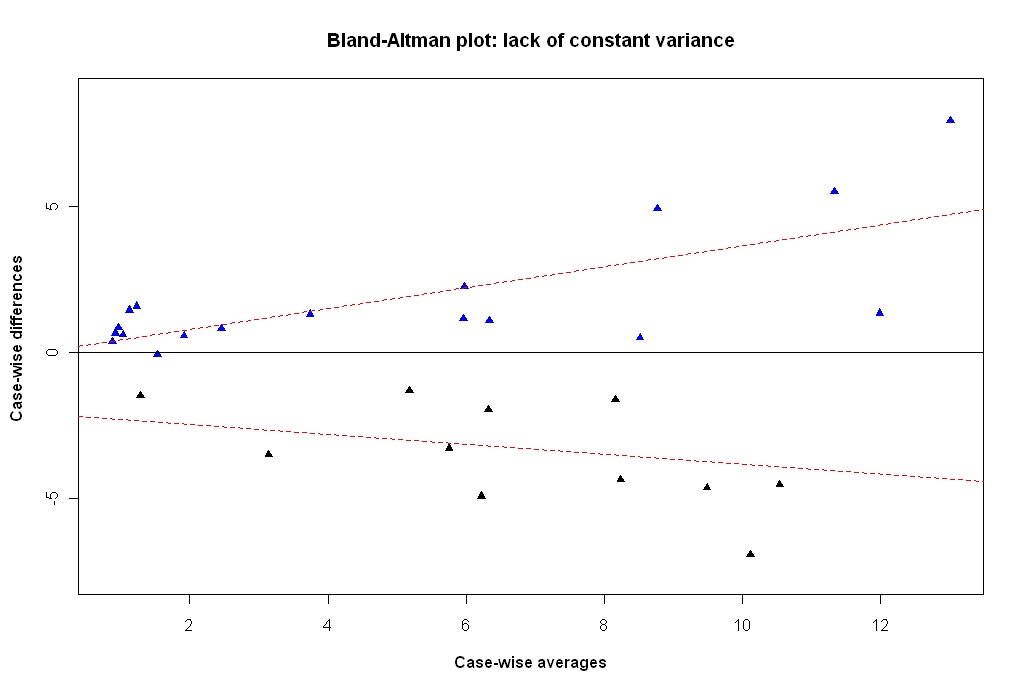
\includegraphics[height=70mm]{BAFanEffect.jpeg}
  \caption{Bland-Altman plot demonstrating the increase of variance over the range.}\label{BAFanEffect}
\end{center}
\end{figure}

\begin{figure}[h!]
\begin{center}
  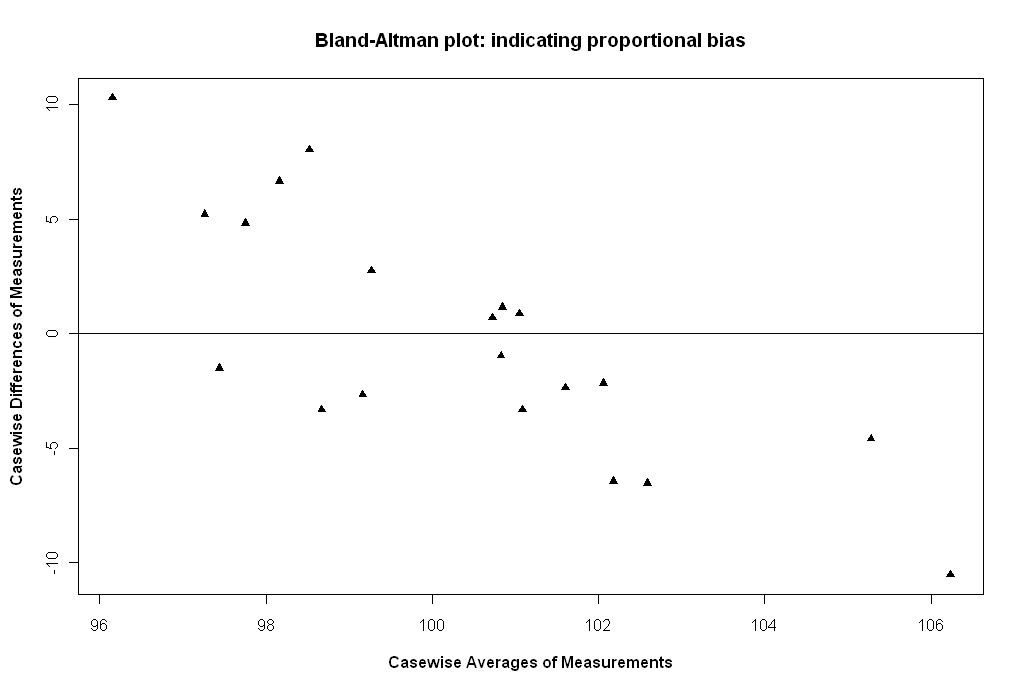
\includegraphics[height=90mm]{PropBias.jpeg}
  \caption{Bland-Altman plot indicating the presence of proportional bias.}\label{PropBias}
\end{center}
\end{figure}
\end{frame}
%%%%%%%%%%%%%%%%%%%%%%%%%%%%%%%%%%%%%%%%%%%%%%%%%%%%%%%%%%%%%%%%%%%%%%%%%%%%%%%%%%%%%%
\begin{frame}
\begin{figure}[h!]
\begin{center}
  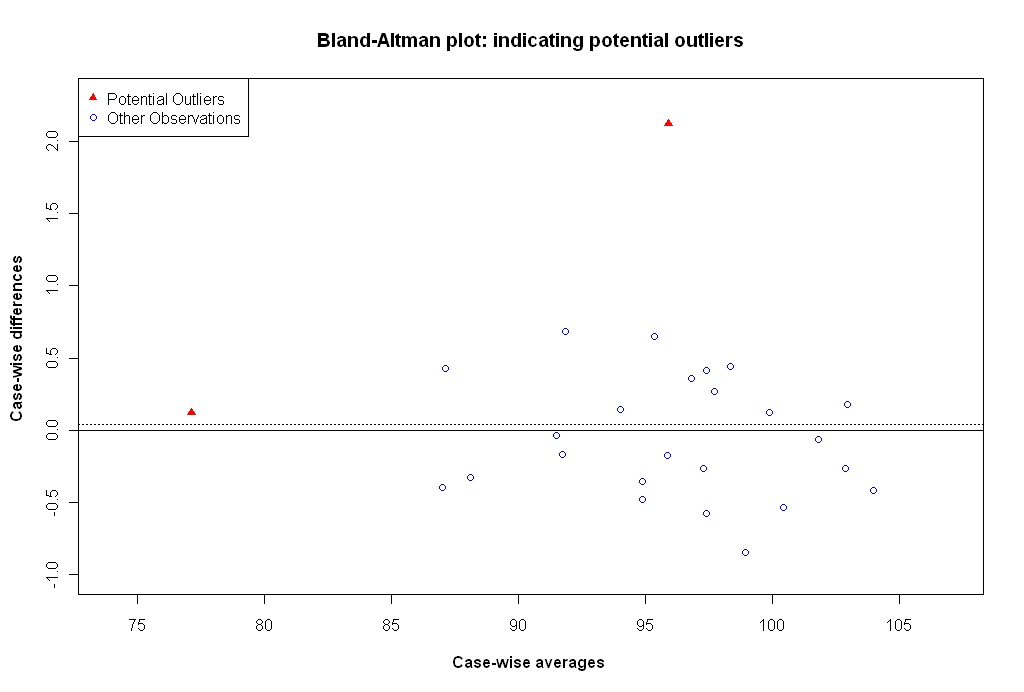
\includegraphics[width=100mm]{BAOutliers.jpeg}
  \caption{Bland-Altman plot indicating the presence of potential outliers.}\label{Outliers}
\end{center}
\end{figure}

\end{frame}

%------------------------------------------------%
\begin{frame}

\frametitle{Live Demonstration}

Live Demonstration of Method Comparison Analysis on Grubbs Data with 
\begin{itemize}
\item Agreement 
\item MethComp 
\end{itemize}

\end{frame}


%------------------------------------------------%

\begin{frame}
\frametitle{\texttt{
Agreement} }
\textbf{Agreement}\\
 Statistical Tools for Measuring Agreement\\ \vspace{0.3cm}

This package computes several statistics for measuring agreement, for example, mean square deviation (MSD), total deviation index (TDI) or concordance correlation coefficient (CCC). \\ \vspace{0.2cm} It can be used for both continuous data and categorical data for multiple raters and multiple readings cases.

\begin{description}
\item[Author]	BYue Yu AND Lawrence Lin
\item[Maintainer]	Yue Yu <yyu at imyy.net>
\item[License]	GPL-2
\item[URL]	http://imyy.net
\end{description}

\end{frame}
%------------------------------------------------%
\begin{frame}
\frametitle{\texttt{MethComp} }
\textbf{MethComp}:  \\ Functions for analysis of agreement in method comparison studies
\\ \vspace{0.2cm}
Methods (standard and advanced) for analysis of agreement between measurement methods.


\begin{description}
\item[Author]	Bendix Carstensen, Lyle Gurrin, Claus Ekstrom, Michal Figurski
\item[Maintainer]	Bendix Carstensen <bxc at steno.dk>
\item[License]	GPL-2 | GPL-3 
\item[URL]	http://BendixCarstensen.com/MethComp/
\end{description}

\end{frame}

%%%%%%%%%%%%%%%%%%%%%%%%%%%%%%%%%%%%%%%%%%%%%%%%%%%%%%%%%%%%%%%%%%%%%%%%%%%%%%%%%%%%%%
\section{Replicate Measurements}
%------------------------------------------------------------------------%

\begin{frame}{\bf \tcb{Replicate Measurements}}
\begin{itemize}\itemsep0.7cm
\item Bland and Altman's approach originally devised for a single measurement on each item by each of the methods.
\item Their 1999 paper [3] extended their approach to replicate measurements:\\ \emph{By replicates we mean two or more measurements on the same
individual taken in identical conditions. \\In general this requirement means that the
measurements are taken in quick succession. }
\item Emphasis put on "repeatability".
\end{itemize}
\end{frame}
\begin{frame}
\frametitle{Limits of Agreement with Replicates}
\begin{itemize}
%\item Computing limits of agreement features prominently in many method comparison studies, further to Bland And Altman's Work}
\item Bland Altman 1999 addresses the issue of computing LoAs in the presence of replicate measurements, suggesting several computationally simple approaches. When repeated measures data are available, it is desirable to use
all the data to compare the two methods. 
\item However, the original Bland-Altman method was developed for two sets of measurements done on one occasion (i.e. independent data), and so this approach is not suitable for replicate measures data. 
%However, as a naive analysis, it may be used to explore the data because of the simplicity of the method.
%\citet{bxc2008} 
\item Bland and Altman [3] address this problem by offering two different
approaches. 
\end{itemize}
\end{frame}

\begin{frame}
\begin{itemize}

\item The premise of the first approach is that replicate
measurements can be treated as independent measurements. 
\item The
second approach is based upon using the mean of the each group of
replicates as a representative value of that group. 
\item Using either
of these approaches will allow an analyst to estimate the inter
method bias.

\item Carstensen et al [4,5] and Roy [6] computes the limits of agreement to the case with replicate measurements by using LME models.
\end{itemize}
\end{frame}

\begin{frame}
\frametitle{Limits of Agreement with Replicates}
\begin{itemize}
\item Carstensen et al [5] takes issue with the limits of agreement based on
mean values, in that they can only be interpreted as prediction
limits for difference between means of repeated measurements by
both methods, as opposed to the difference of all measurements.
Incorrect conclusions would be caused by such a misinterpretation.
\item Carstensen et al [5] demonstrates how the limits of agreement
calculated using the mean of replicates are `much too narrow as
prediction limits for differences between future single
measurements'. 
%\item This paper also comments that, while treating the
%replicate measurements as independent will cause a downward bias
%on the limits of agreement calculation, this method is preferable
%to the `mean of replicates' approach.
\end{itemize}
\end{frame}
%-------------------------------------------------------------------------------------%
\begin{frame}
\frametitle{Limits of Agreement with Replicates}
\begin{itemize}
%\item This paper seeks to use Roy's approach to estimate the limits of agreement. These estimates will be compared to estimates computed under Carstensen's formulation.

\item In computing limits of agreement, it is first necessary to have an estimate for the standard deviations of the differences. 
\item When the agreement of two methods is analyzed using LME models, a clear method of how to compute the standard deviation is required. 
\item Different approaches in fitting LME models will yield different results.
\item As the estimate for inter-method bias and the quantile would be the same under various approaches, the focus is solely on the standard deviation.
\end{itemize}
\end{frame}


%%%%%%%%%%%%%%%%%%%%%%%%%%%%%%%%%%%%%%%%%%%%%%%%%%%%%%%%%%%%%%%%%%%%%%%%%%%%%%%%%%%%%%
%\subsection*{Limits of Agreement}
%\begin{frame}
%\begin{itemize}
%\item  However, the original Bland-Altman method was developed for two sets of measurements done on one occasion (i.e. independent data), and so this approach is not suitable for replicate measures data.
%\item However, as a naive analysis, it may be used to explore the data because of the simplicity of the method.
%\end{itemize}
%\end{frame}
%\textit{\begin{frame}
%
%
%Thus far, the formulation for comparison of two measurement
%methods is one where one measurement by each method is taken on
%each subject. Should there be two or more measurements by each
%methods, these measurement are known as `replicate measurements'.
%\alert{BXC2008} recommends the use of replicate measurements, but
%acknowledges that  additional computational complexity.
%\end{frame}
%}
%%%%%%%%%%%%%%%%%%%%%%%%%%%%%%%%%%%%%%%%%%%%%%%%%%%%%%%%%%%%%%%%%%%%%%%%%%%%%%%%%%%%%%

%%%%%%%%%%%%%%%%%%%%%%%%%%%%%%%%%%%%%%%%%%%%%%%%%%%%%%%%%%%%%%%%%%%%%%%%%%%%%%%%%%%%%%

%--------------------------------------------------------------------- %
%---------------------------------------------------------------------------------------%
\begin{frame}
\frametitle{Limits of Agreement}
\begin{itemize}
\item Carstensen et al [5] computes the limits of agreement to the case with replicate measurements by using LME models.
\item Roy [6] formulates a very powerful method of assessing whether two methods of measurement, with replicate measurements, also using LME models. 
\item Roy's approach is based on the construction of variance-covariance matrices.
\item Importantly, Roy's approach does not directly address the issue of limits of agreement (although another related analysis , the \emph{Coefficient of Repeatability}, is mentioned).
\end{itemize}
\end{frame}

\end{document}